\chapter{Исследовательский раздел}
В данном разделе будет проведено исследование зависимости времени исполнения запроса к базе данных от наличия индексации столбцов базы. Будет показан график, отображающий зависимость времени исполнения от индексации. В этом разделе также будут приведены технические характеристики устройства, на котором выполнялось измерение.

\section{Технические характеристики}
Тестирование выполнялось на устройстве со следующими техническими характеристиками:
\begin{itemize}
	\item операционная система Ubuntu 20.04.3 LTS [8];
	\item память 7.5 GiB;
	\item процессор Intel(R) Core(TM) i7-8550U CPU @ 1.80GHz × 8 [9].
\end{itemize}

Во время тестирования устройство было подключено к блоку питания и не нагружено никакими приложениями, кроме встроенных приложений окружения, окружением и системой тестирования.

\section{Постановка эксперимента}

\textbf{Цель эксперимента} --- оценка времени исполнения запроса к базе данных с использованием индексации и без нее.

Оценка будет производиться для таблицы Product. Измеряться будет время поиска в данной таблице по полю title, оно же и будет проиндексировано.

\section{Результаты эксперимента}

В таблице \ref{time-table} представлены результаты тестов.

\captionsetup{singlelinecheck = false, justification=raggedright}
\begin{table}[h!]
	\begin{center}
		\caption{Время исполнения запроса в зависимости от использования индексации}
		\begin{tabular}{ |c|c|c|c| }
			\hline
			\textbf{\specialcell{Количество \\записей в таблице}} & \textbf{\specialcell{Без индексации}} & \textbf{\specialcell{С индексацией}}\\ \hline
			100 & 0.058 & 0.043\\ \hline
			250 & 0.121 & 0.048\\ \hline
			500 & 0.184 & 0.055\\ \hline
			750 & 0.247 & 0.069\\ \hline
			1000 & 0.361 & 0.081\\ \hline
		\end{tabular}
		\label{time-table}
	\end{center}
\end{table}			

На рисунке \ref{index} представлен график зависимости времени исполнения запроса и использованием индексации и без нее от количества записей в таблице.

\captionsetup{singlelinecheck = false, justification=centering}
\begin{figure}[h!]
	\begin{center}
		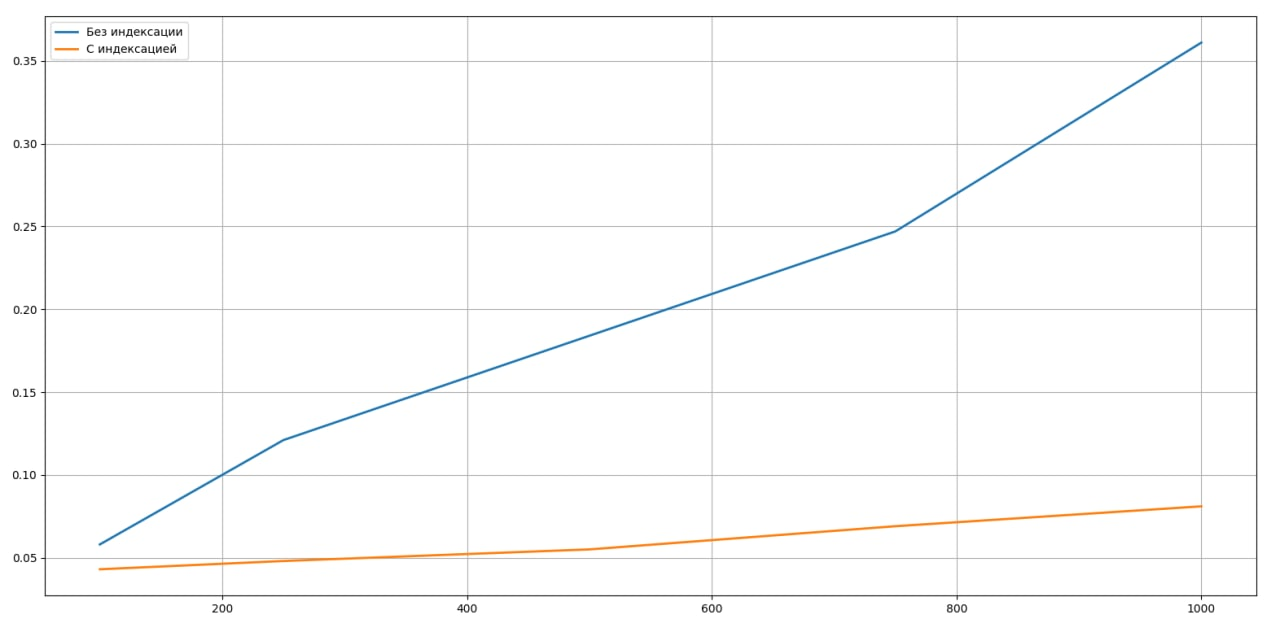
\includegraphics[scale=0.5]{assets/index.jpg}
	\end{center}
	\caption{График зависимости времени запроса от индексации}
	\label{index}
\end{figure}

\section*{Вывод}
\addcontentsline{toc}{section}{Вывод}
По результатам эксперимента можно сделать вывод, что индексация существенно сокращает время ответа. При небольшой заполненности таблицы(100 записей) выигрыш по времени составляет 26\%. При заполненности в 1000 записей выигрыш составляет 78\%.


